% OmniMed-FL --- corrected/audited submission draft.
% Results and figures are generated from the validated reviewer merge
% (experiments/reviewer_results_merged.json). Figures under omnimed_plots/
% belong to the withdrawn pre-audit runs and must not be included here.
\documentclass[letterpaper, conference]{IEEEtran}
\IEEEoverridecommandlockouts

% Strict margin enforcement and text wrapping
\usepackage[letterpaper, top=0.75in, bottom=1in, left=0.625in, right=0.625in]{geometry}
\usepackage{microtype}

\usepackage{cite}
\usepackage{amsmath,amssymb,amsfonts}
\usepackage{graphicx}
\usepackage{textcomp}
\usepackage{xcolor}
\usepackage{booktabs}
\usepackage{url}
\usepackage{placeins}
\usepackage{balance}
% \usepackage{stfloats}  % not installed in all TeX distributions; no [b] figure* is used
\usepackage{tikz}
\usetikzlibrary{arrows.meta,shapes.geometric,positioning,fit,backgrounds,calc}

\definecolor{llmblue}   {RGB}{76,114,176}
\definecolor{vitgreen}  {RGB}{85,168,104}
\definecolor{vlmred}    {RGB}{196,78,82}
\definecolor{fedorange} {RGB}{204,185,116}
\definecolor{fedpurple} {RGB}{129,114,178}
\definecolor{outyyellow}{RGB}{255,242,204}
\definecolor{smallgray} {RGB}{220,220,220}

% Only generated/ (validated) figures are on the graphics path.
\graphicspath{{generated/}}

\tikzset{
  mainbox/.style={draw, rounded corners=4pt, align=center,
                  minimum height=0.75cm, text width=#1,
                  font=\footnotesize, inner sep=4pt},
  mainbox/.default=2.4cm,
  llmbox/.style ={mainbox, fill=llmblue!30,  draw=llmblue!80!black},
  vitbox/.style ={mainbox, fill=vitgreen!30, draw=vitgreen!80!black},
  vlmbox/.style ={mainbox=5.2cm, fill=vlmred!25, draw=vlmred!80!black,
                  minimum height=1.0cm},
  fedbox/.style ={mainbox=1.9cm, fill=fedpurple!40, draw=fedpurple!80!black},
  outbox/.style ={mainbox=4.5cm, fill=outyyellow, draw=yellow!70!black},
  sbox/.style   ={draw, rounded corners=2pt, fill=smallgray,
                  minimum height=0.5cm, align=center,
                  font=\scriptsize, inner sep=3pt, text width=1.8cm},
  arr/.style    ={-{Stealth[length=5pt]}, thick},
  darr/.style   ={-{Stealth[length=5pt]}, thick, dashed},
}

\begin{document}
\renewcommand{\arraystretch}{0.85}
\setlength{\abovecaptionskip}{0pt}
\setlength{\belowcaptionskip}{0pt}

% Tight but standard float separation.
\setlength{\textfloatsep}{8pt plus 2pt minus 2pt}
\setlength{\dbltextfloatsep}{8pt plus 2pt minus 2pt}
\setlength{\intextsep}{8pt plus 2pt minus 2pt}
\setlength{\floatsep}{8pt plus 2pt minus 2pt}
\setlength{\dblfloatsep}{8pt plus 2pt minus 2pt}

\setlength{\columnsep}{0.25in}

\renewcommand{\dbltopfraction}{0.95}
\renewcommand{\topfraction}{0.95}
\renewcommand{\textfraction}{0.05}
\renewcommand{\floatpagefraction}{0.75}
\renewcommand{\dblfloatpagefraction}{0.75}

\title{OmniMed-FL: A Robust Multimodal Federated Learning Framework for Clinical Diagnosis}

\author{
\IEEEauthorblockN{$^1$Ayush Debnath, $^{2,3,4}$Ruelia Saha, $^{2}$Sudip Misra}

\IEEEauthorblockA{$^1$Department of Mechanical Engineering\\
Indian Institute of Technology Kharagpur, India 721302}

\IEEEauthorblockA{$^2$Department of Computer Science and Engineering\\
Indian Institute of Technology Kharagpur, India 721302}

\IEEEauthorblockA{$^3$KTH Royal Institute of Technology, Stockholm, Sweden}

\IEEEauthorblockA{$^4$SRM University-AP, India}

Emails: \{ayush.d@kgpian.iitkgp.ac.in, ruelia.saha.rs@gmail.com, sudipm@iitkgp.ac.in\}
}

\maketitle

\begin{abstract}
Simultaneous assessment of medical imaging and patient records is required in
clinical diagnosis. But standard machine learning pipelines cannot analyze these
several sorts of data together. Meanwhile, HIPAA and GDPR preclude hospitals from
aggregating sensitive patient data centrally. This leaves a crucial void: secure
fusion of visual and textual context across distant networks. We present OmniMed-FL,
a controlled systems study of multimodal federated learning for five-class clinical
condition classification (Normal, Pneumonia, COVID-19, Pleural Effusion,
Cardiomegaly). Our proxy corpus pairs 2,400 public chest radiographs and 600
synthetic COVID-19 surrogates with 3,000 class-conditioned synthetic notes, matched by
class, not by patient. The framework benchmarks eight fusion strategies,
three initializations, four missing-text imputation rules, and matched federated
baselines under non-IID Dirichlet partitioning across 3 to 20 hospital clients.
Because all notes and the COVID-19 images are synthetic and pairing is not
patient-level, these are descriptive proxy comparisons, not estimates of diagnostic
performance or deployment readiness. Within those limits: at $K{=}5$ and severe skew
($\alpha{=}0.1$), local-only training achieves a macro-F1 score of 0.310, FedAvg
achieves $0.652\!\pm\!0.057$, FedProx $0.685\!\pm\!0.064$, a matched FedMME-style
one-shot ensemble $0.537\!\pm\!0.217$, and our SCAFFOLD--AdamW adaptation
$0.192\!\pm\!0.129$, the 0.033 FedProx--FedAvg gap falling inside either two-seed
standard deviation. Over a $4\!\times\!3$ grid, label skew costs up to 0.28 F1
(0.874--0.896 at $\alpha{=}5$ against 0.615--0.741 at $\alpha{=}0.1$) whereas a
near-sevenfold client increase costs at most 0.13, while bidirectional volume grows
linearly to 183.5\,GiB at $K{=}20$. A branch audit is starker: multimodal
concatenation spends $2.3\times$ the model state of a text-only branch scoring 0.111 F1
higher.
\end{abstract}

\begin{IEEEkeywords}
Multimodal Federated Learning, Vision--Language Models, Clinical Condition
Classification, E-Health, Non-Identically Distributed Data, Communication Cost,
Retrieval
\end{IEEEkeywords}

% ─────────────────────────────────────────────────────────────────────────────
\section{Introduction}
% ─────────────────────────────────────────────────────────────────────────────

\IEEEPARstart{C}{linical} prediction improves when a radiograph is read alongside
the text filed with it, and a centralized model can do that, provided somebody is
permitted to pool the data. Frequently nobody is. Federated learning (FL) avoids
the pooling step by exchanging parameter updates instead of
examples~\cite{Rajpurkar2017,Irvin2019,McMahan2017}, although keeping raw records at
home is a data-locality property, not a privacy proof.

Federated medical imaging is well trodden by
now~\cite{Sheller2020,Dou2021,Kaissis2021}, and so is centralized medical
vision--language modeling. Their intersection is not. Put the two together and four
questions arrive at once: how badly does label skew hurt, when does a five-class head
collapse onto its majority class, which fusion operator earns its compute, and what
does a multimodal model cost to move. OmniMed-FL
answers those four for a controlled proxy benchmark, and we would rather be blunt
about scope up front. Our radiographs and synthetic notes are not patient matched,
so we measure the learning system, not clinical diagnosis. ``Robust'' here means
stress tests across partitions, client counts, and missing modalities, not a
clinical guarantee.

\subsection{Contribution}
\begin{itemize}
\item Our contribution is a protocol, not another fusion operator. Heterogeneity,
client count, anti-collapse components, initialization, and eight fusion rules all
run inside one federated loop that fixes the corpus, partition draw, shard profile,
encoders, optimizer, and local budget, so a difference between arms is a difference
in the named factor and nothing else.
\item We add matched controls for two recent multimodal FL methods: a FedMME-style
one-shot ensemble, at both our 24-epoch and FedMME's native 100-epoch budget, and a
P-FIN-style missing-text stress test over four imputation rules.
\item We report the systems side that accuracy tables usually omit: realized
per-client skew, GPU-synchronized round time, peak memory, formula-derived
bidirectional FP32 volume, and retrieval over all 600 validation queries.
\item We publish the null results too. The fusion sweep, the FedProx--FedAvg gap,
and most anti-collapse contrasts at moderate skew come out smaller than their own
two-seed spreads, and we say so rather than rank them.
\end{itemize}


% ─────────────────────────────────────────────────────────────────────────────
\section{Related Work}

\subsection{Medical Image Classification}
Early automated diagnostics treated the chest radiograph as a pure computer-vision
problem. CheXNet and CheXpert set the centralized CNN
baselines~\cite{Rajpurkar2017,Irvin2019}, and Vision Transformers later showed that
global context helps on the same task~\cite{Dosovitskiy2021,Liu2021swin}. All of them
pool data on one server, and none reads the note a clinician wrote next to the image.

\subsection{Federated Clinical Learning}
To stay inside privacy regulation, the clinical community moved to FL: FedAvg for
decentralized training~\cite{McMahan2017}, multi-institutional collaboration without
sharing patient records~\cite{Sheller2020}, multinational COVID-19 CT
validation~\cite{Dou2021}, and privacy-enhanced image learning~\cite{Kaissis2021}.
FedProx and SCAFFOLD attack the client heterogeneity that degrades naive
averaging~\cite{Li2020fedprox,Karimireddy2020}; clinical variants add prompt
aggregation, split hybrids, architecture search, personalization, label-scarce
transfer, distillation, foundation models, and hardened
privacy~\cite{Zhao2025fedlppa,Mao2025fedsplit,Zhang2024fednas,Jiang2025apfl,Wang2024ftl,Li2024globecom,Ahmed2025feddistill,Huang2025globecom,Yang2025fedfm,Dvornek2024review,Zhou2024ppvit,Chen2024globecom,Sun2024globecom}. These frameworks train across
distributed hospitals, but stay strictly unimodal.

\subsection{Vision--Language Models in Healthcare}
Concurrently, BiomedCLIP, LLaVA-Med, and MedCLIP aligned radiographs with reports and
demonstrated what fusion
buys~\cite{Zhang2023biomedclip,Li2023llavamed,Wang2022medclip}, on centralized corpora
no single hospital can assemble. Multimodal FL is only now catching up: FedMME votes
over one-shot client ensembles, and P-FIN imputes missing features with calibrated
uncertainty~\cite{Wang2025fedmme,Shahid2026pfin}, and federated clinical VLMs are
only now appearing~\cite{Yan2024crossmodal,Akkaya2024fedvlm,Zhang2024globecom}.

\textbf{Synthesis.} The gap is not that nobody has combined the two halves. It is
that the papers which do sit on different datasets, backbones, and budgets, which
makes their headline scores incomparable. So we rebuild FedMME- and P-FIN-style arms
inside our own loop as matched adaptations, and never quote a score across papers.
Holding everything but one factor fixed is what earns the results: it is why we can
attribute the one-shot deficit to aggregation rather than to FedMME's larger local
budget, and why an eight-way fusion sweep that looks decisive turns out to be noise.

% ─────────────────────────────────────────────────────────────────────────────
\section{System Design}
% ─────────────────────────────────────────────────────────────────────────────

\subsection{Architecture}

Figure~\ref{fig:arch} lays out the pipeline. We tokenize notes with WordPiece at
a 128-token cap, resize radiographs to $224{\times}224$, and normalize them
against ImageNet statistics. The DistilBERT~\cite{Sanh2019} \texttt{[CLS]} vector
is projected to $\mathbf{h}_t\!\in\!\mathbb{R}^{256}$, and mean-pooled ViT tokens
give $\mathbf{h}_v\!\in\!\mathbb{R}^{512}$. Eight lightweight operators then
merge the two: projected concatenation, residual cross-attention, gated residual
fusion, dual-projection concatenation, a one-layer decoder A, a distinct
two-query/two-layer decoder B, non-residual 384-dimensional cross-attention, and
a two-token Transformer encoder. Some code keys still carry foundation-model names
from an earlier iteration; they are compact fusion rules, not implementations of
those models. All eight feed the same two-layer, five-class multilayer perceptron
(MLP) and share the data, partition, optimizer, and local budget. The question we
wanted to settle was narrow: can a cheap projection hold its own against heavier
attention machinery on hardware a hospital actually owns?


\begin{figure}[t]
\centering
\resizebox{0.98\columnwidth}{!}{%
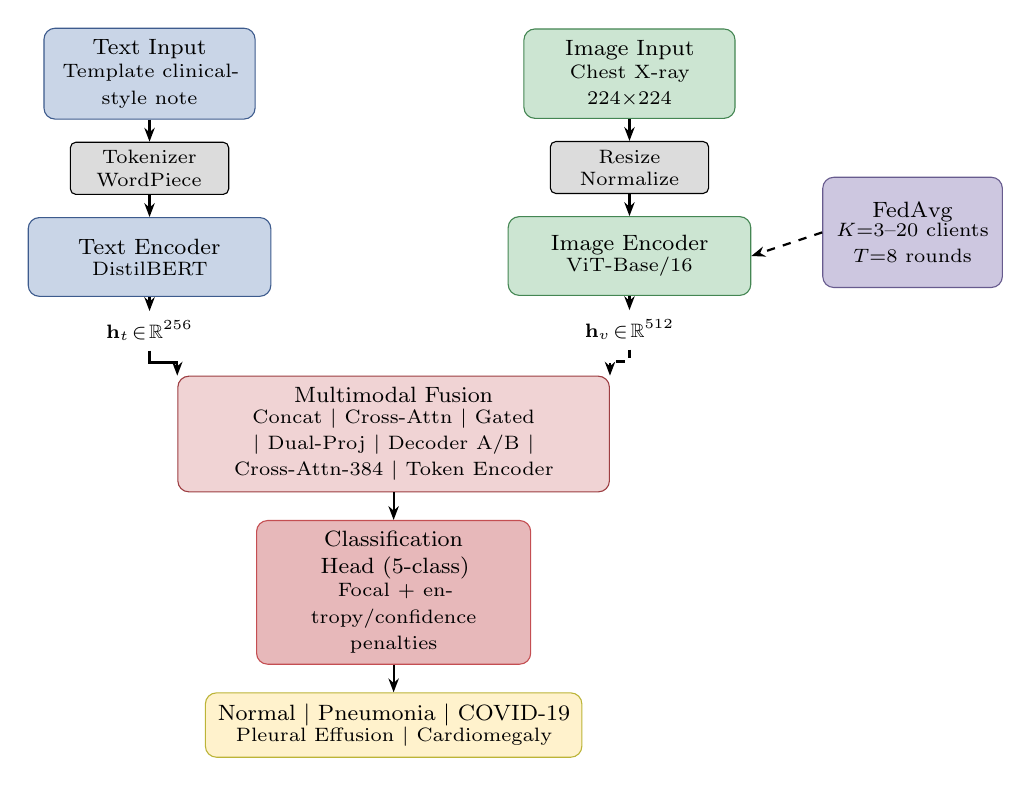
\begin{tikzpicture}[node distance=0.45cm]
  \node[llmbox] (ti)  {Text Input\\[-1pt]{\scriptsize Template clinical-style note}};
  \node[sbox, below=0.28cm of ti] (tok) {Tokenizer\\WordPiece};
  \node[llmbox, below=0.28cm of tok, text width=2.8cm, minimum height=1.0cm]
        (llm) {Text Encoder\\[-2pt]{\scriptsize DistilBERT}};
  \node[font=\scriptsize, below=0.18cm of llm] (ht)
        {$\mathbf{h}_t\!\in\!\mathbb{R}^{256}$};

  \node[vitbox, right=3.4cm of ti] (ii) {Image Input\\[-1pt]
                                         {\scriptsize Chest X-ray $224{\times}224$}};
  \node[sbox, below=0.28cm of ii] (aug) {Resize\\Normalize};
  \node[vitbox, below=0.28cm of aug, text width=2.8cm, minimum height=1.0cm]
        (vit) {Image Encoder\\[-2pt]{\scriptsize ViT-Base/16}};
  \node[font=\scriptsize, below=0.18cm of vit] (hv)
        {$\mathbf{h}_v\!\in\!\mathbb{R}^{512}$};

  \node[fedbox, right=0.9cm of vit, yshift=0.3cm, minimum height=1.4cm,
        text width=2.0cm] (fed)
        {FedAvg\\[-1pt]{\scriptsize $K{=}3$--20 clients\\$T{=}8$ rounds}};

  \node[vlmbox, below=1.0cm of llm, xshift=3.1cm, minimum height=0.95cm]
        (vlm) {Multimodal Fusion\\[-2pt]
               {\scriptsize Concat $|$ Cross-Attn $|$ Gated $|$ Dual-Proj $|$
               Decoder A/B $|$ Cross-Attn-384 $|$ Token Encoder}};

  \node[mainbox=3.2cm, fill=vlmred!40, draw=vlmred,
        below=0.35cm of vlm] (cls)
        {Classification Head (5-class)\\[-1pt]
         {\scriptsize Focal + entropy/confidence penalties}};

  \node[outbox, below=0.35cm of cls] (out)
        {Normal $|$ Pneumonia $|$ COVID-19\\[-2pt]
         {\scriptsize Pleural Effusion $|$ Cardiomegaly}};

  \draw[arr](ti)--(tok);\draw[arr](tok)--(llm);\draw[arr](ii)--(aug);
  \draw[arr](aug)--(vit);\draw[arr](llm)--(ht);\draw[arr](vit)--(hv);
  \draw[arr](ht.south)--++(0,-0.15)-|(vlm.north west);
  \draw[darr](hv.south)--++(0,-0.15)-|(vlm.north east);
  \draw[arr](vlm)--(cls);\draw[arr](cls)--(out);
  \draw[darr](fed.west)--(vit.east);
\end{tikzpicture}%
}
\caption{OmniMed-FL architecture. DistilBERT and ViT-Base/16 encode the two
proxy modalities; lightweight multimodal fusion combines them; FedAvg
coordinates simulated clients without exchanging their raw examples.}
\label{fig:arch}
\end{figure}

\subsection{Federated and Local Objectives}
\label{sec:objective}
Let $K$ clients hold disjoint shards $\mathcal{D}_k$ of the training split, with
$n_k=|\mathcal{D}_k|$ and $n=\sum_k n_k$, and let $\theta$ collect the trainable
parameters on the fusion path: both encoders, the projection layers, the fusion
operator, and the classification head. We minimize the sample-weighted empirical
risk
\begin{equation}
\begin{aligned}
\min_{\theta}\ F(\theta)&=\sum_{k=1}^{K}\frac{n_k}{n}F_k(\theta),\\[-2pt]
F_k(\theta)&=\frac{1}{n_k}\!\!\sum_{(x,z,y)\in\mathcal{D}_k}\!\!\ell\big(f_\theta(x,z),y\big).
\end{aligned}
\label{eq:fedobj}
\end{equation}
where $x$ is a radiograph, $z$ its class-paired note, $y$ the class label, and
$f_\theta$ the fused five-class classifier. Shards never leave a client, and the
server sees only the trainable tensors listed above. For mini-batch
$\mathcal{B}$, the loss we actually implement is
\begin{equation}
\ell_{\mathcal B}=\frac{1}{|\mathcal B|}\sum_{i\in\mathcal B}
(1-p_{i,y_i})^{\gamma}\mathrm{CE}_{\epsilon,i}
+\lambda\phi(h)+5[q-0.9]_+,
\label{eq:loss}
\end{equation}
with $p_{i,y_i}$ the true-class probability, $\mathrm{CE}_{\epsilon,i}$
label-smoothed cross-entropy, $\gamma{=}2$, $\epsilon{=}0.05$, $C{=}5$,
$h=H(\bar p)/\log C$, $q=|\mathcal B|^{-1}\sum_i\max_c p_{ic}$,
$\phi(h)=(1-h)[1-\tfrac{8}{3}[h-0.7]_+]$, and $[u]_+=\max(u,0)$.
The entropy-diversity term grows whenever a batch's predictions concentrate, and we
attenuate it above normalized entropy 0.7 so it stops pushing once the head is
healthy. Setting $\lambda{=}0$ removes that term alone, while the confidence
penalty $5[q-0.9]_+$ stays fixed everywhere. The class-balanced sampler and the
entropy-diversity term are the two anti-collapse components we ablate in
Section~\ref{sec:results}. Predicted-class diversity is the fraction of the five
labels that ever appear as a validation-set argmax.

Each round, the server broadcasts $\theta^{(t)}$, every eligible client runs three
local AdamW epochs on class-balanced mini-batches under~\eqref{eq:loss}, clips the
gradient norm at one, and returns its trainable tensors for the sample-weighted
update in~\eqref{eq:fedobj}. Operational runs start from public DistilBERT and
ViT-Base/16 weights with random task heads. We fine-tune both encoders and keep
unused unimodal heads and the inactive CNN fallback out of optimization and
communication.

\subsection{Controlled Proxy Corpus}

\textbf{Image data.}
We built a balanced 3,000-image proxy corpus at 600 examples per class. The public
radiographs come from the Kermany pneumonia collection~\cite{Kermany2018} and the NIH
ChestX-ray dataset~\cite{Wang2017chestxray8}, and our loader logs verify 2,400 public
images spanning Normal, Pneumonia, Pleural Effusion, and Cardiomegaly. The COVID-19
source we originally specified was unavailable when the runs executed, so the 600
COVID-19 images are synthetic X-ray-style surrogates carrying bilateral opacity
patterns, which leaves the image axis partly confounded with source collection and
synthetic status. All images are resized to
$224{\times}224$, ImageNet-normalized, shuffled deterministically, and split 80/20
into 2,400 training and 600 validation examples.

\textbf{Clinical text data.}
No patient electronic health record (EHR) data are used. Real EHR text is hard to
source publicly, so we wrote a template engine instead. It pairs each image label, at
the class level, with a synthetic clinical-style note assembled from observation,
symptom, context, and indicator slots. To keep the network from memorizing an
obvious keyword we engineered the mix deliberately: 25\% of notes
draw every slot from the target class, 35\% mix target and non-target slots, and
40\% are heavily mixed while retaining a probabilistic target-class indicator.
This cuts direct label wording, but image and note do not come from the same
patient and must never be described as a real image--report pair.

\label{sec:corpus}
\textbf{What the corpus does and does not support.}
Every arm sees the same controlled corpus, which is what makes our internal
comparisons meaningful. The absolute scores are another matter. Templates can leave
shortcuts, label-level pairing strips out the discordance and missingness of real
records, our surrogates may not resemble clinical COVID-19 radiographs, and the split
is grouped by neither patient nor source.

\subsection{Experimental Setup}

\textbf{Hyperparameters.}
Table~\ref{tab:hyper} collects the protocol. Every client trains with AdamW at
learning rate $10^{-4}$ and weight decay $0.01$ for three local epochs per round.
The suite runs eight rounds at batch size 16 in FP32, without automatic mixed
precision (AMP). Our reference setting is five clients at Dirichlet $\alpha=1.0$,
and Section~\ref{sec:results} varies $\alpha$ and the client count explicitly. Seeds
0 and 1 drive initialization, sampling, and partitioning, with one exception:
pooled-start reuses a single seed-0 checkpoint under seed-specific FL partitions. We
ran everything in PyTorch on one NVIDIA H100 NVL device in a server we share with
unrelated workloads. The GPU-synchronized timer wraps sequential local training and
aggregation within a round, and excludes validation, setup, I/O, networking,
concurrency, and multi-node throughput. Our timings are an execution-cost record,
not distributed throughput. We also did not force deterministic CUDA algorithms, so
a seed fixes the software pseudorandom streams without buying identical reruns.

\textbf{Partitioning.}
For each class, a Dirichlet draw allocates training indices across clients. Smaller
$\alpha$ concentrates client label distributions, and $\alpha\!\to\!\infty$
approaches independent and identically distributed (IID)
allocation~\cite{Hsu2019}. A nominal $\alpha$ does not fully describe a finite split,
so we report the per-client class shares we actually drew alongside our scalability
results. The split is fixed across rounds for a given seed. Shards
holding fewer than four examples skip local optimization but still contribute the
unchanged global state at their sample weight. We do not renormalize over active
clients, which is why our cells report active alongside nominal $K$.

\textbf{Matched recent-method controls.}
Our FedMME-style arm uploads each client model once and applies equal-weight hard
voting, breaking ties by mean softmax~\cite{Wang2025fedmme}. We run it at two local
budgets. Our matched 24 epochs isolates the method from the budget; FedMME's native
100 epochs removes the budget discrepancy. Reporting both keeps the two confounds
separate. Either way it keeps the common corpus,
shard profile, encoders, and optimizer, substituting our five-class inputs for
FedMME's generated-report pipeline. The P-FIN-style stress test fixes
three multimodal and two image-only clients, projects both encoders to
256-dimensional normalized features, and compares zero filling, deterministic FIN,
Gaussian $\beta$-negative-log-likelihood ($\beta$-NLL) imputation ($\beta{=}0.5$),
and uncertainty-weighted aggregation with Fed-UQ-Avg balance weight 0.6 and
temperature 0.2~\cite{Shahid2026pfin}. We kept concatenation instead of P-FIN's
bidirectional cross-modal attention: with one pooled feature per modality,
cross-attention carries unit weight and collapses to a linear projection. FedProx uses $\mu{=}0.01$.

\textbf{Why these settings.}
Within an ablation family, only the named factor moves. Three local epochs across
eight rounds give a tractable 24-local-epoch budget, and batch size 16 is simply what
holds both encoders plus one local model copy in GPU memory for the largest FP32
model. The grid crosses $K{=}\{3,5,10,20\}$ with $\alpha{=}\{0.1,1,5\}$ and the
$K{=}5$ sweep adds $\alpha{=}0.3$ and $0.5$, so the study spans severe to near-IID
skew; $K{=}5$ is our small cross-silo reference and $K{=}3$--20 probes count
sensitivity. Two seeds support descriptive claims, not significance. Everything else
in Table~\ref{tab:hyper} is a fixed default, not a per-model optimum.

\begin{table}[t]
\caption{Common simulation parameters.}
\label{tab:hyper}
\centering\footnotesize
\setlength{\tabcolsep}{4pt}
\begin{tabular}{llll}
\toprule
\textbf{Parameter} & \textbf{Value} & \textbf{Parameter} & \textbf{Value} \\
\midrule
Local Epochs ($E$)   & 3      & Seeds                    & 0, 1 \\
Fed.\ Rounds ($T$)   & 8      & Grid $K$ (ref.)          & 3, 5, 10, 20 (5) \\
Batch Size           & 16     & Grid $\alpha$ (ref.)     & 0.1, 1, 5 (1) \\
AdamW LR             & $10^{-4}$ & $K{=}5$ extra $\alpha$ & 0.3, 0.5 \\
Weight Decay         & $0.01$ & Precision                & FP32, no AMP \\
Diversity wt.\ ($\lambda$) & 1.0 & Init.                & Public enc.\ + rand.\ heads \\
\bottomrule
\end{tabular}
\end{table}

\section{Results}
\label{sec:results}

\begin{figure*}[!t]
\centering
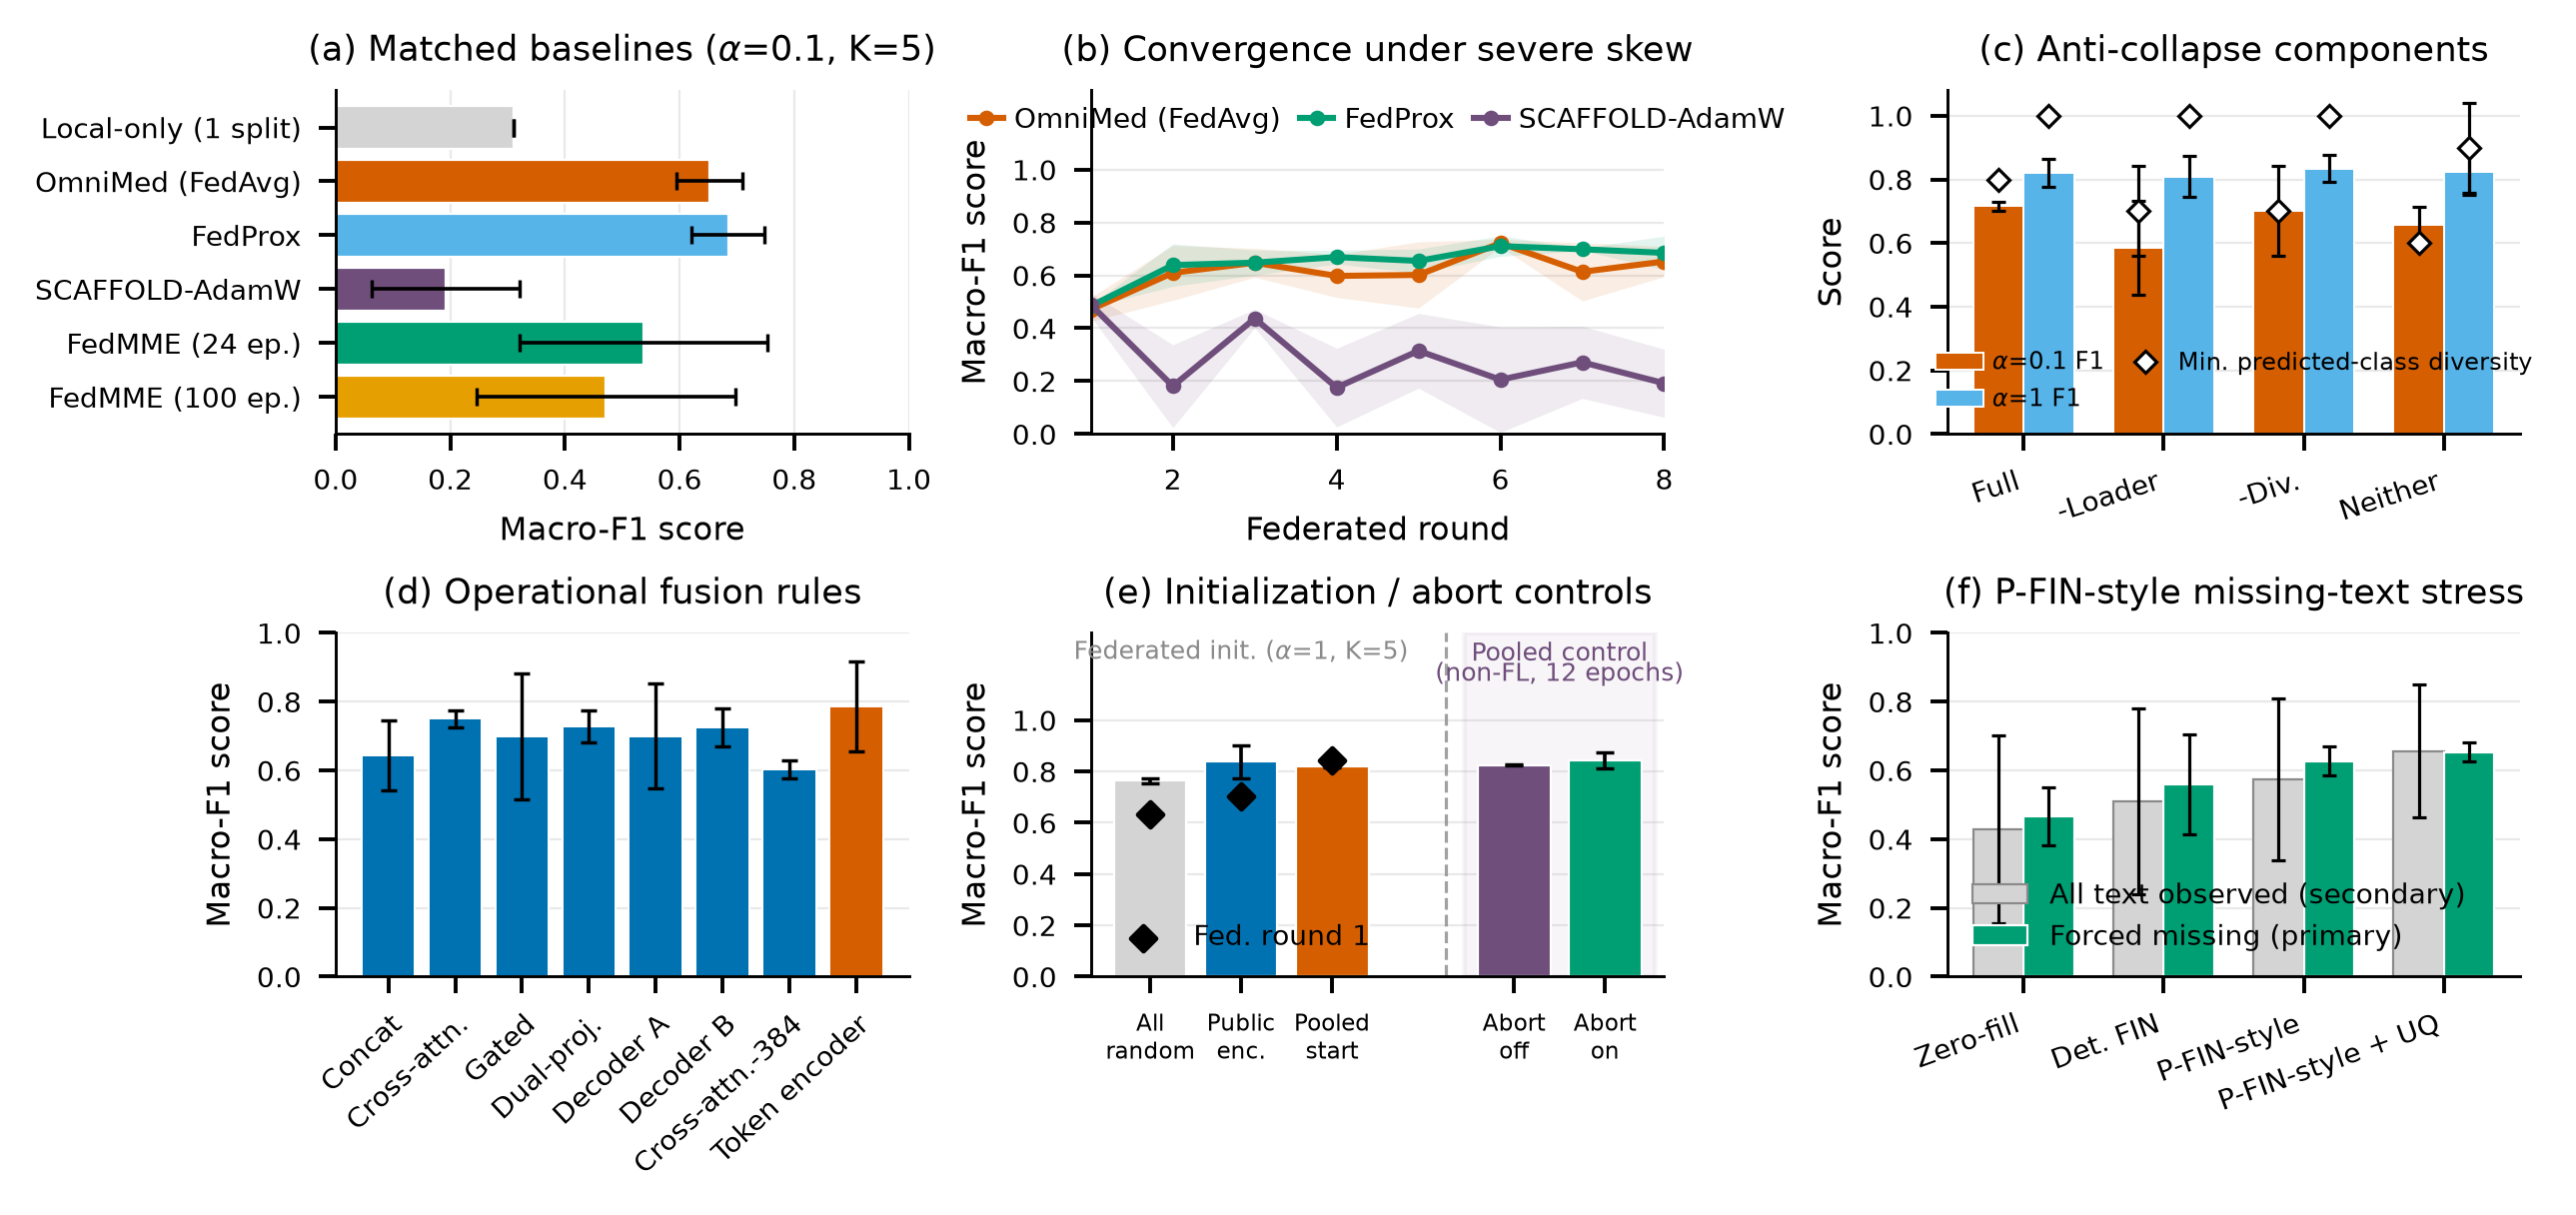
\includegraphics[width=0.81\textwidth,height=4.05in,keepaspectratio]{reviewer_matched_results}
\caption{Matched results (two-seed mean$\pm$SD unless noted). (a)~Severe-skew
baselines; local-only is a five-client mean from one partition, iterative arms use
$8$ rounds of $3$ epochs. (b)~Iterative convergence. (c)~Anti-collapse F1, diamonds
for minimum predicted-class diversity. (d)~Eight fusion rules trained in-loop at
$\alpha{=}0.1$. (e)~Federated initialization (round-1 diamonds) and separated
non-federated abort controls, whose trigger never fires. (f)~P-FIN-style adaptation;
held-out text forced missing for the primary metric.}
\label{fig:matched}
\end{figure*}

\subsection{Matched Baselines under Severe Skew}

Every arm in Fig.~\ref{fig:matched}(a) shares the corpus, partition draw, encoders,
and optimizer at $\alpha{=}0.1$, $K{=}5$; all but the native-budget FedMME arm also
share the 24-local-epoch budget. Local-only training averages a macro-F1 score of
0.310 across the five clients of one partition. Over
two matched seeds, FedAvg reaches $0.652\!\pm\!0.057$ and FedProx
$0.685\!\pm\!0.064$. Their 0.033 gap is smaller than either sample standard
deviation, so these runs do not separate the two methods and we will not pretend
otherwise. Our SCAFFOLD--AdamW adaptation lands at $0.192\!\pm\!0.129$, and the
oscillation in panel~(b) points at our AdamW control-variate adaptation rather than
at classical SGD-based SCAFFOLD. The FedMME-style arm trains five client models
independently and combines them by equal-weight hard voting with mean-softmax ties. At our matched 24-epoch budget it reaches
$0.537\!\pm\!0.217$ (seeds 0.690, 0.384), and at FedMME's native 100-epoch budget
it reaches $0.472\!\pm\!0.225$ (seeds 0.631, 0.312). Quadrupling local computation
does not close the gap to iterative aggregation, so the gap belongs to one-shot
aggregation under severe skew, not to a budget handicap. Both budgets are our most
seed-sensitive arms for a structural reason: one aggregation has no later round in
which to repair a poor local solution. Every arm except SCAFFOLD--AdamW clears
local-only training, though the overlapping intervals make that a coarse ordering
rather than a ranking.

\subsection{Anti-Collapse, Fusion, and Initialization Ablations}

Under severe skew the full class-balanced-sampler and entropy-diversity stack
reaches $0.716\!\pm\!0.014$ F1 at minimum predicted-class diversity 0.8. Drop the
sampler, the entropy-diversity term, or both, and F1 falls to
$0.585\!\pm\!0.148$, $0.701\!\pm\!0.011$, and $0.657\!\pm\!0.057$, with minimum
diversity $0.7\!\pm\!0.14$, $0.7\!\pm\!0.14$, and $0.6\!\pm\!0.00$
(Fig.~\ref{fig:matched}(c)). The sampler is the larger and more
variance-reducing of the two, and only the full stack keeps four of five classes
predicted every round. The confidence penalty in \eqref{eq:loss} stays fixed
across all four arms. At $\alpha{=}1$ the same four configurations land within
$0.809$--$0.834$ with every minimum diversity at or above 0.9. These components earn
their place under severe skew and are close to inert at moderate skew. One more
observation: three suites nominally repeat the same severe-skew
FedAvg/concatenation setting, yet return $0.652\!\pm\!0.057$, $0.674\!\pm\!0.185$,
and $0.716\!\pm\!0.014$, differing by more than their own spreads. We report them
separately rather than pool them or quote the flattering one.

Panel~(d) trains all eight fusion rules inside the operational federated loop. The
means run from $0.603$ for non-residual 384-dimensional cross-attention up to
$0.787$ for the two-token Transformer encoder, with per-rule sample standard
deviations of $0.024$--$0.183$. Since the widest interval exceeds the entire
between-rule spread, the sweep cannot rank fusion operators, and we will not. Projected concatenation, our default everywhere else, sits mid-pack at
$0.643\!\pm\!0.102$.

Panel~(e) separates three federated initializations at $\alpha{=}1$. The all-random arm
keeps both architectures but initializes every weight from scratch, opening at 0.635
round-1 F1 and closing at $0.765\!\pm\!0.010$. Public
encoders with random task modules, our operational default, open at 0.704 and close
at $0.839\!\pm\!0.065$. Pooled-start reuses one seed-0 checkpoint from a 12-epoch
centralized run for both FL seeds, so its pretraining sits outside the shared
budget; it opens far higher at 0.843 and ends lower at $0.818\!\pm\!0.004$. Public encoders
buy roughly 0.07 F1 over random initialization; the pooled checkpoint buys a round-1
head start that does not survive to round~8. It was also selected on the
reporting validation split, making it a diagnostic, not an unbiased generalization
estimate. Non-federated abort-off/on
controls post epoch-12 F1 of $0.825\!\pm\!0.001$ and $0.843\!\pm\!0.032$, best-epoch
$0.845\!\pm\!0.013$ and $0.884\!\pm\!0.003$, on pooled data with sampling and
diversity off. All complete 12 epochs at diversity 1.0, so the branch never fires and
the gap is rerun variation.

Panel~(f) is our matched P-FIN-style adaptation, where 256-dimensional
$L_2$-normalized features and concatenation plus an MLP replace the source
bidirectional-attention stack. On the primary forced-missing-text metric the four
imputation rules order consistently: zero filling $0.465\!\pm\!0.084$, deterministic
FIN $0.559\!\pm\!0.144$, Gaussian $\beta$-NLL imputation $0.627\!\pm\!0.042$, and
uncertainty-weighted aggregation $0.653\!\pm\!0.027$. The ordering holds in both
seeds, and the spread tightens as the method models its own uncertainty, the
qualitative behavior P-FIN reports. The secondary all-text-observed scores are far
noisier, $0.429$--$0.657$ with SD up to $0.274$, so missing text is the
better-determined comparison.

\begin{figure}[!t]
\centering
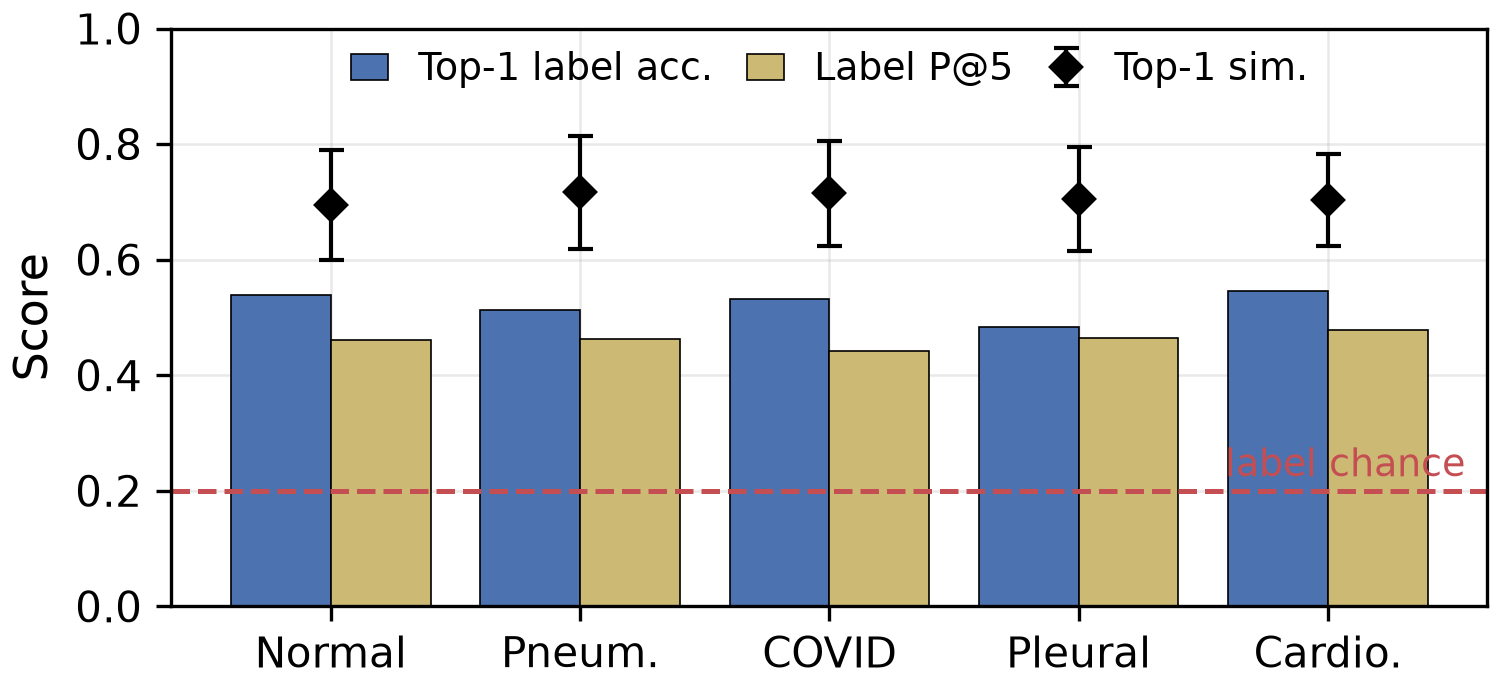
\includegraphics[width=0.98\columnwidth,height=1.34in,keepaspectratio]{fig_rag_validated}
\caption{FAISS exact inner-product retrieval over 2,400 indexed training-note
vectors for 600 validation-note queries; TF--IDF is fitted on training notes only.
Bars show top-1 same-label accuracy and same-label precision@5; diamonds show mean
top-1 cosine similarity with population-SD whiskers. The dashed 0.2 line is a
five-class label prior, not a similarity baseline; this evaluates retrieval, not
generation.}
\label{fig:retrieval}
\end{figure}

\subsection{Retrieval-Stage Evaluation for Retrieval-Augmented Generation (RAG)}

Exact inner-product FAISS search~\cite{Johnson2021faiss} over training-fitted
TF--IDF note vectors gives condition-macro averages of 0.522 for top-1 same-label
retrieval accuracy, 0.459 for same-label precision@5, and 0.707 for mean top-1
cosine similarity, with the five condition rows covering all 600 validation
queries (Fig.~\ref{fig:retrieval}). Top-1 accuracy sits well above the 0.2
five-class label prior yet far below the 0.707 mean similarity. That combination is
the signature of a template corpus: neighbors come out lexically close whether or
not they share a label. This check is neither a fine-tuned DistilBERT result nor a
generated-answer evaluation, and it establishes no clinical retrieval quality.

\begin{figure*}[!t]
\centering
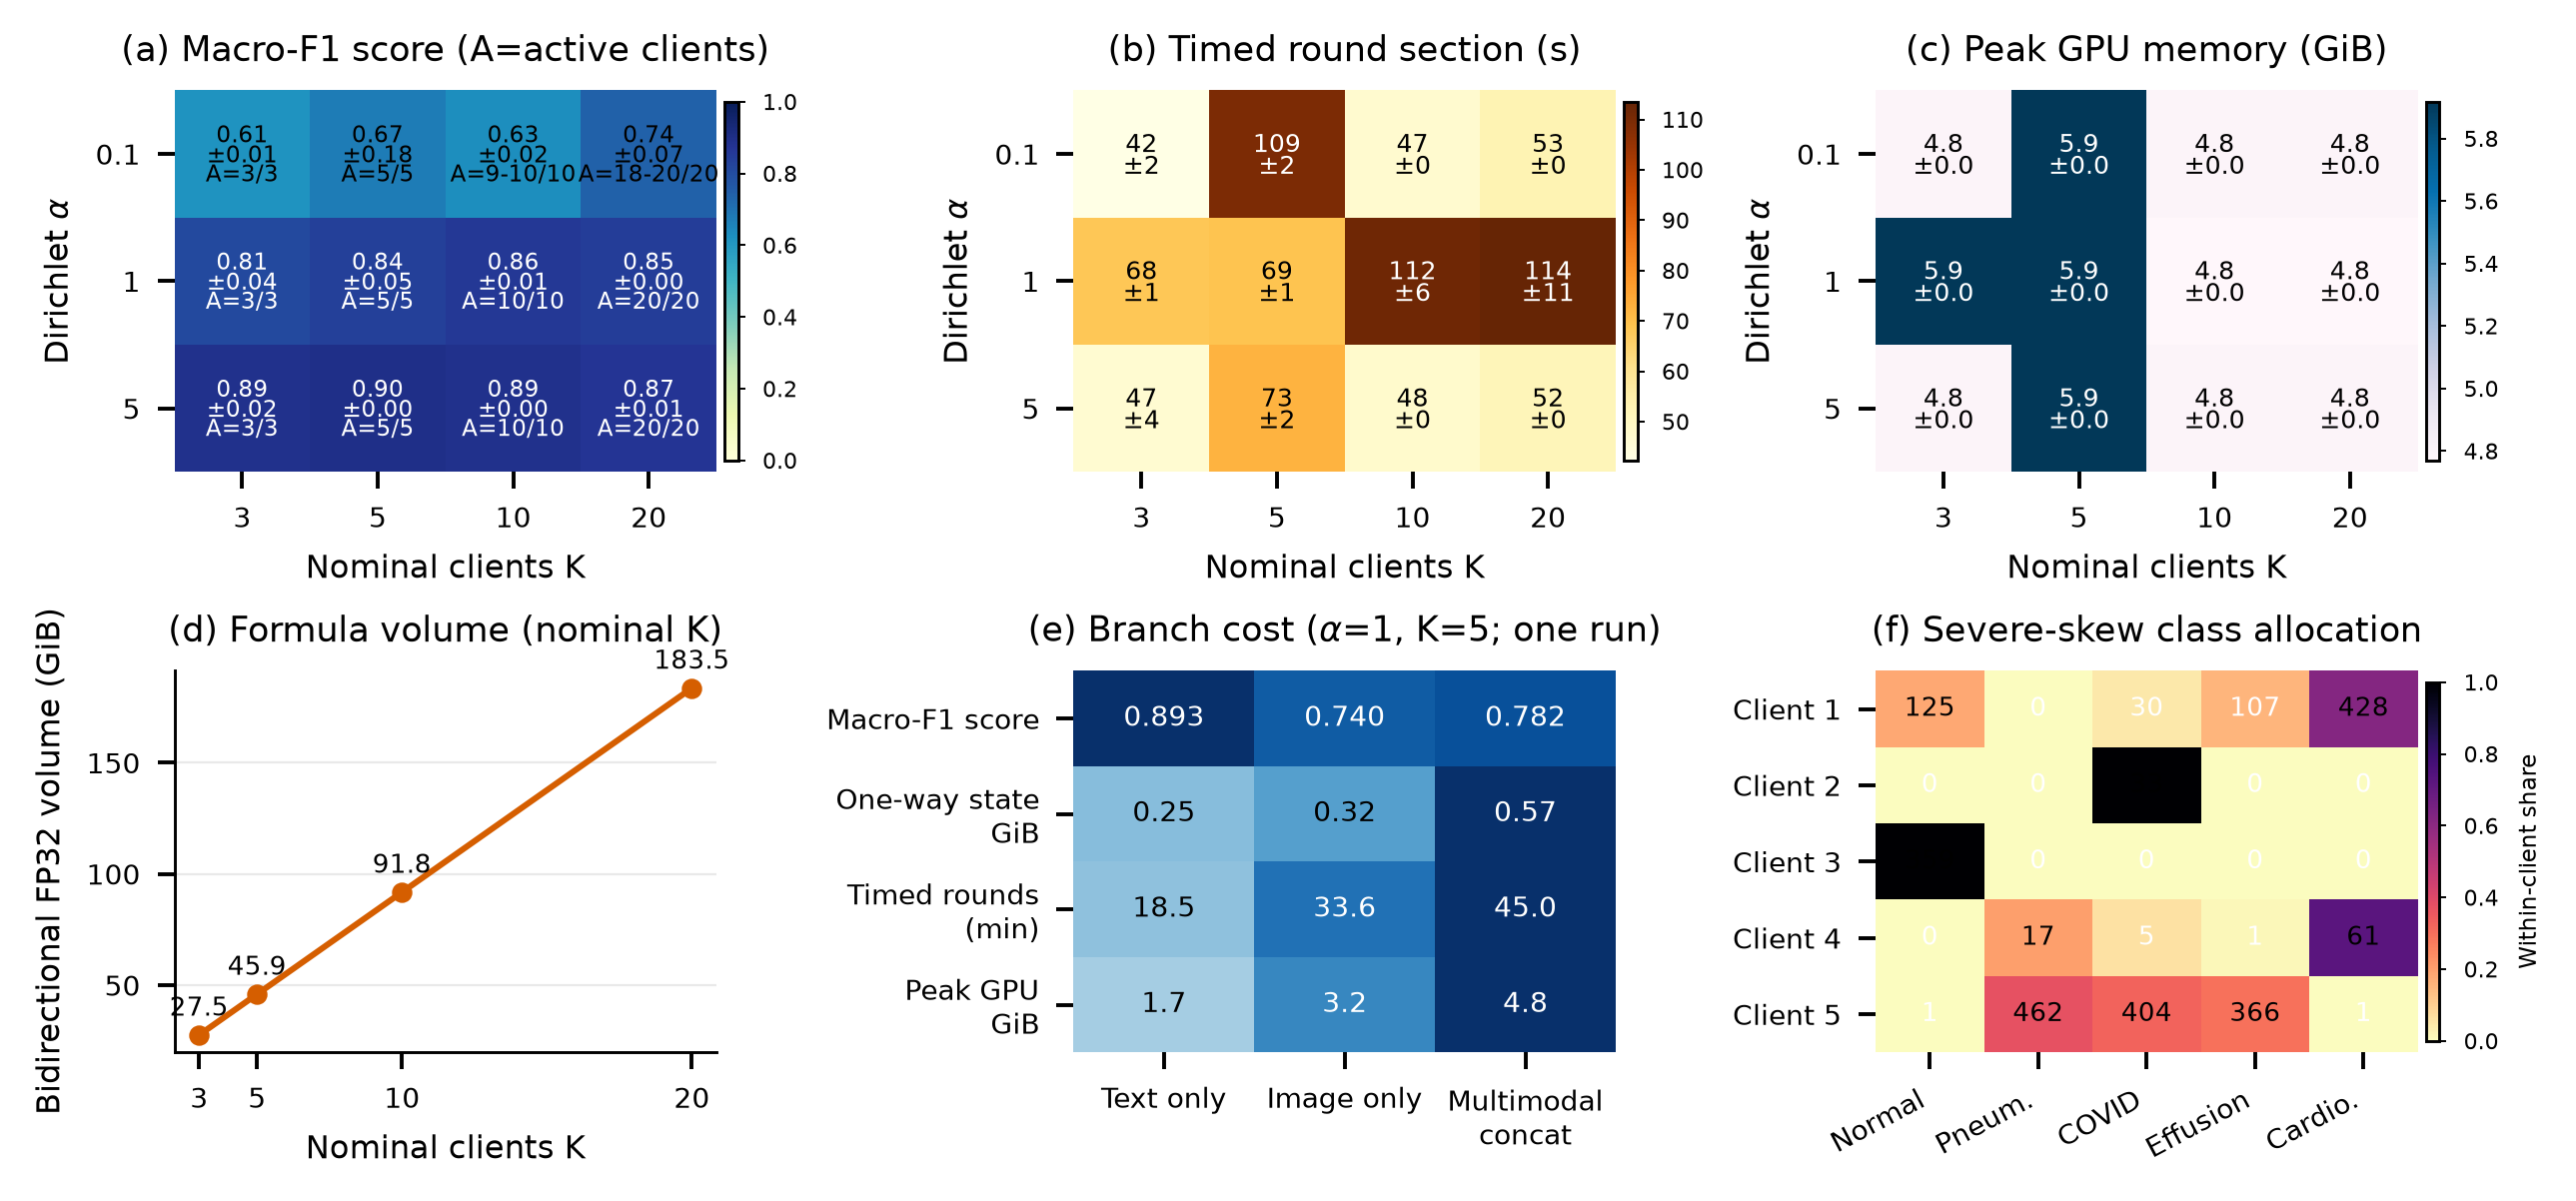
\includegraphics[width=0.81\textwidth,height=4.05in,keepaspectratio]{reviewer_systems_scalability}
\caption{Scalability/resource audit. Two-seed mean$\pm$SD for (a)~macro-F1 score
($A/K$ is active/nominal clients), (b)~the GPU-synchronized training/aggregation
section per round, and (c)~peak allocated memory within it. (d)~Formula FP32 volume
over eight rounds, skipped shards included; not measured traffic. (e)~One-run branch
cost at $\alpha{=}1,K{=}5$. (f)~Severe-skew seed-0 counts.}
\label{fig:systems}
\end{figure*}

\subsection{Scalability, Communication, and Resource Cost}

Figure~\ref{fig:systems}(a) assembles the full Cartesian product of
$K{=}\{3,5,10,20\}$ and $\alpha{=}\{0.1,1,5\}$, and one factor dominates
throughout: label skew, not client count. Every $\alpha{=}5$ cell lies in
$0.874$--$0.896$ and every $\alpha{=}1$ cell in $0.812$--$0.863$, whereas the
$\alpha{=}0.1$ row drops to $0.615$--$0.741$ with far wider spreads, up to
$\pm0.185$ at $K{=}5$. Within a row, moving $K$ by a factor of nearly seven shifts
the mean by at most 0.13 F1, and the $\alpha{=}0.1$ row is not even monotone in
$K$. Our auxiliary $K{=}5$ checks at $\alpha{=}0.3$ and $0.5$ give
$0.769\!\pm\!0.043$ and $0.824\!\pm\!0.113$. Cells report $A/K$, where $A$ counts
clients whose realized shard reaches four samples: allocation is complete except
under severe skew, where $K{=}10$ retains 9--10 and $K{=}20$ retains 18--20 active
clients. Panel~(f) shows the realized per-client class counts behind one
severe-skew cell, where single clients hold entire classes.

Panels~(b) and~(c) report runtime and peak allocated memory for the timed block on
one shared H100 NVL. Timed sections span 42--114\,s per round and peak memory
4.77--5.92\,GiB. Neither panel is a scaling curve: the $K{=}5$ column and the
$\alpha{=}1$ row are inherited from our earlier validated suite and ran in a
different session, which produces the 5.92\,GiB cells and the slowest timed sections.
Sequential simulation and contention, not client count, explain the rest.

For $|\theta|$ trainable parameters, $b$ bytes/parameter, $T$ rounds, and
nominal $K$, the plotted bidirectional volume is
\begin{equation}
V_{\mathrm{nom}}=2KT|\theta|b,
\label{eq:comm}
\end{equation}
Here $|\theta|{=}153{,}935{,}621$, $b{=}4$, and $T{=}8$, so a 615,742,484-byte
model state gives nominal bidirectional volumes of 27.5/45.9/91.8/183.5\,GiB at
$K{=}3/5/10/20$ ($1$ GiB$=2^{30}$ bytes). We keep the nominal count when $A{<}K$;
swapping $A$ for $K$ is an alternative estimate, not a measurement. Serialization,
headers, retransmission, secure aggregation, compression, and algorithm-specific
state all sit outside it. Panel~(d) puts the
operating point plainly. Communication grows linearly in $K$ while accuracy stays
nearly flat in $K$. At $\alpha{=}5$, going from $K{=}3$ to $K{=}20$ buys a 0.014 F1
change for $6.7\times$ the traffic.

The one-run branch audit in panel~(e) is where the multimodal bill comes due.
Text, image, and multimodal F1 are 0.893/0.740/0.782, one-way FP32 model-state
sizes are 0.248/0.324/0.573\,GiB, sums of timed round durations are
18.5/33.6/45.0\,min, and peak allocated memory is 1.69/3.18/4.77\,GiB. Multimodal
concatenation costs $2.3\times$ the model state, $2.4\times$ the wall time, and
$2.8\times$ the memory of the text branch, and it scores 0.111 F1 below that branch.
One run per branch cannot support a blanket claim of multimodal superiority, and we
suspect a mundane cause: class-conditioned template shortcuts that the text encoder
can exploit directly.

\section{Discussion and Limitations}

Partition sensitivity is the finding that survives everything we threw at it: at
$\alpha{=}0.1$, even identically configured FedAvg reruns move substantially. Three
boundaries hem in what that buys a deployment. First, our client-count study is a
sequential simulation on a shared server. It models neither concurrent workers,
latency, stragglers, and dropout nor heterogeneous accelerators, and we never test
aggregation against poisoned or Byzantine updates. Our own dispersion hints at why
that is hard: at $\alpha{=}0.1$ honest updates already spread by $\pm0.185$ F1, so a
trimmed-mean or median aggregator must discard genuine minority-class signal to
reject an adversarial one, while sample-weighted FedAvg leaves a large shard
unbounded leverage. Skew and Byzantine tolerance pull against each other, and
quantifying that needs a threat model we did not build. Our title's ``robust'' denotes
these stress tests, nothing stronger. Second, communication.
Eq.~\eqref{eq:comm} exposes model-state scaling and Fig.~\ref{fig:systems}(e) the
multimodal footprint, but a real study would measure end-to-end traffic and latency
under compression, partial participation, and failures. We implement neither secure
aggregation nor the differentially private training of
Abadi~\textit{et al.}~\cite{Abadi2016}. Keeping raw examples local is a locality
property, not a privacy guarantee.

Third, clinical interpretation stays bounded by Section~\ref{sec:corpus}. Neither our
absolute F1 nor our retrieval scores estimate diagnostic safety, generalization,
clinical utility, or deployment readiness, and with two seeds our spreads are
descriptive rather than significant. What we want next is not a longer version of
this study but a different one: larger multi-site datasets, more seeds,
native-method replications, calibrated uncertainty, and privacy testing.

\section{Conclusion}

OmniMed-FL is a controlled systems study of multimodal FL, not a clinical
validation. Across a $4\times3$ client-count/skew grid, eight fusion rules, three
initializations, four missing-text imputation rules, and matched FedAvg, FedProx,
SCAFFOLD--AdamW, and FedMME-style baselines, one result holds consistently. Label
skew dominates. Client count is near-neutral for accuracy and linear in
communication. Everything else is conditional on the partition realization and our
protocol choices. Real patient-paired data and safeguards come before clinical use, and we would rather publish the null results
than imply we have cleared that bar.



\FloatBarrier
\bibliographystyle{IEEEtran}
\let\oldbibliography\thebibliography
\renewcommand{\thebibliography}[1]{%
  \oldbibliography{#1}%
  \fontsize{6.3}{6.9}\selectfont
  \setlength{\itemsep}{0pt}%
  \setlength{\parskip}{0pt}%
  \setlength{\parsep}{0pt}%
  \setlength{\topsep}{0pt}%
  \setlength{\labelsep}{3pt}%
  \linespread{0.90}\selectfont
}

\section*{Acknowledgment}
This work was supported in part by the Indian National Academy of Engineering
(INAE) Chair Professorship grant awarded to the third author.

\balance
\begin{thebibliography}{99}

\bibitem{Rajpurkar2017}
P.~Rajpurkar, J.~Irvin, K.~Zhu, \emph{et al.}, ``CheXNet: Radiologist-level
pneumonia detection on chest X-rays with deep learning,'' \emph{arXiv:1711.05225},
2017.

\bibitem{Irvin2019}
J.~Irvin, P.~Rajpurkar, M.~Ko, \emph{et al.}, ``CheXpert: A large chest radiograph
dataset with uncertainty labels and expert comparison,'' in \emph{Proc. AAAI Conf.
Artif. Intell.}, vol.~33, 2019, pp.~590--597.

\bibitem{McMahan2017}
H.~B. McMahan, E.~Moore, D.~Ramage, S.~Hampson, and B.~Ag{\"u}era y~Arcas,
``Communication-efficient learning of deep networks from decentralized data,'' in
\emph{Proc. Int. Conf. Artif. Intell. Statist.}, vol.~54, 2017, pp.~1273--1282.

\bibitem{Sheller2020}
M.~J. Sheller, B.~Edwards, G.~A. Reina, \emph{et al.}, ``Federated learning in
medicine: Facilitating multi-institutional collaborations without sharing patient
data,'' \emph{Sci. Rep.}, vol.~10, art.~12598, 2020.

\bibitem{Dou2021}
Q.~Dou, T.~Y. So, M.~Jiang, \emph{et al.}, ``Federated deep learning for detecting
COVID-19 lung abnormalities in CT: A privacy-preserving multinational validation
study,'' \emph{npj Digit. Med.}, vol.~4, art.~60, 2021.

\bibitem{Kaissis2021}
G.~Kaissis, A.~Ziller, J.~Passerat-Palmbach, \emph{et al.}, ``End-to-end privacy
preserving deep learning on multi-institutional medical imaging,'' \emph{Nature
Mach. Intell.}, vol.~3, no.~6, pp.~473--484, 2021.

\bibitem{Dosovitskiy2021}
A.~Dosovitskiy, L.~Beyer, A.~Kolesnikov, \emph{et al.}, ``An image is worth
16$\times$16 words: Transformers for image recognition at scale,'' in \emph{Proc.
Int. Conf. Learn. Represent.}, 2021.

\bibitem{Liu2021swin}
Z.~Liu, Y.~Lin, Y.~Cao, \emph{et al.}, ``Swin Transformer: Hierarchical vision
transformer using shifted windows,'' in \emph{Proc. IEEE/CVF Int. Conf. Comput.
Vis.}, 2021, pp.~10012--10022.

\bibitem{Li2020fedprox}
T.~Li, A.~K. Sahu, M.~Zaheer, \emph{et al.}, ``Federated optimization in
heterogeneous networks,'' in \emph{Proc. Mach. Learn. Syst.}, vol.~2, 2020,
pp.~429--450.

\bibitem{Karimireddy2020}
S.~P. Karimireddy, S.~Kale, M.~Mohri, \emph{et al.}, ``SCAFFOLD: Stochastic
controlled averaging for federated learning,'' in \emph{Proc. Int. Conf. Mach.
Learn.}, vol.~119, 2020, pp.~5132--5143.

\bibitem{Zhang2023biomedclip}
S.~Zhang, Y.~Xu, N.~Usuyama, \emph{et al.}, ``BiomedCLIP: A multimodal biomedical
foundation model pretrained from fifteen million scientific image-text pairs,''
\emph{arXiv:2303.00915}, 2023.

\bibitem{Li2023llavamed}
C.~Li, C.~Wong, S.~Zhang, \emph{et al.}, ``LLaVA-Med: Training a large
language-and-vision assistant for biomedicine in one day,'' in \emph{Proc. Adv.
Neural Inf. Process. Syst.}, vol.~36, 2023, pp.~28541--28564.

\bibitem{Wang2022medclip}
Z.~Wang, Z.~Wu, D.~Agarwal, and J.~Sun, ``MedCLIP: Contrastive learning from
unpaired medical images and text,'' in \emph{Proc. Conf. Empirical Methods Natural
Lang. Process.}, 2022, pp.~3876--3887.

\bibitem{Wang2025fedmme}
N.~Wang, Y.~Deng, S.~Fan, \emph{et al.}, ``Multi-modal one-shot federated ensemble
learning for medical data with vision large language model,''
\emph{arXiv:2501.03292}, 2025.

\bibitem{Shahid2026pfin}
N.~F. Shahid, M.~Ahmed, M.~A. Haider, \emph{et al.}, ``Probabilistic feature
imputation and uncertainty-aware multimodal federated aggregation,'' in \emph{Proc.
Med. Imag. Deep Learn.}, vol.~315, 2026, pp.~3593--3607.

\bibitem{Sanh2019}
V.~Sanh, L.~Debut, J.~Chaumond, and T.~Wolf, ``DistilBERT, a distilled version of
BERT: Smaller, faster, cheaper and lighter,'' \emph{arXiv:1910.01108}, 2019.

\bibitem{Kermany2018}
D.~S. Kermany, M.~Goldbaum, W.~Cai, \emph{et al.}, ``Identifying medical diagnoses
and treatable diseases by image-based deep learning,'' \emph{Cell}, vol.~172,
no.~5, pp.~1122--1131.e9, 2018.

\bibitem{Wang2017chestxray8}
X.~Wang, Y.~Peng, L.~Lu, \emph{et al.}, ``ChestX-ray8: Hospital-scale chest X-ray
database and benchmarks on weakly-supervised classification and localization of
common thorax diseases,'' in \emph{Proc. IEEE Conf. Comput. Vis. Pattern
Recognit.}, 2017, pp.~2097--2106.

\bibitem{Hsu2019}
T.-M.~H. Hsu, H.~Qi, and M.~Brown, ``Measuring the effects of non-identical data
distribution for federated visual classification,'' \emph{arXiv:1909.06335}, 2019.

\bibitem{Johnson2021faiss}
J.~Johnson, M.~Douze, and H.~J\'egou, ``Billion-scale similarity search with
GPUs,'' \emph{IEEE Trans. Big Data}, vol.~7, no.~3, pp.~535--547, 2021.

\bibitem{Abadi2016}
M.~Abadi, A.~Chu, I.~Goodfellow, \emph{et al.}, ``Deep learning with differential
privacy,'' in \emph{Proc. ACM SIGSAC Conf. Comput. Commun. Secur.}, 2016,
pp.~308--318.

\bibitem{Zhao2025fedlppa}
Y.~Zhao, L.~Wang, T.~Chen, and Q.~Liu, ``FedLPPA: Learning personalized prompt and
aggregation for federated weakly-supervised medical image segmentation,''
\emph{IEEE Trans. Med. Imag.}, vol.~44, no.~3, pp.~1022--1035, 2025.

\bibitem{Mao2025fedsplit}
J.~Mao, J.~Liu, X.~Tian, \emph{et al.}, ``Toward integrating federated learning
with split learning via spatio-temporal graph framework for brain disease
prediction,'' \emph{IEEE Trans. Med. Imag.}, vol.~44, no.~3, pp.~1145--1158, 2025.

\bibitem{Yan2024crossmodal}
Y.~Yan, H.~Wang, Y.~Huang, \emph{et al.}, ``Cross-modal vertical federated learning
for MRI reconstruction,'' \emph{IEEE J. Biomed. Health Informat.}, vol.~28,
no.~11, pp.~6384--6394, 2024.

\bibitem{Zhang2024fednas}
H.~Zhang, X.~Zhang, J.~Lee, \emph{et al.}, ``Generalizable reconstruction for
accelerating MR imaging via federated learning with neural architecture search,''
\emph{IEEE Trans. Med. Imag.}, vol.~43, no.~12, pp.~2314--2327, 2024.

\bibitem{Dvornek2024review}
N.~Dvornek and J.~Ventura, ``Federated learning for multi-site medical image
analysis: A review,'' \emph{Med. Image Anal.}, vol.~92, art.~103045, 2024.

\bibitem{Akkaya2024fedvlm}
F.~Akkaya and B.~Glocker, ``FedVLM: A robust federated vision-language model for
clinical diagnosis,'' \emph{IEEE J. Biomed. Health Informat.}, vol.~28, no.~8,
pp.~4520--4532, 2024.

\bibitem{Jiang2025apfl}
Z.~Jiang, J.~Zheng, and R.~Braren, ``Adaptive personalized federated learning for
COVID-19 detection,'' \emph{IEEE Trans. Neural Netw. Learn. Syst.}, vol.~36,
no.~4, pp.~1870--1882, 2025.

\bibitem{Wang2024ftl}
T.~Wang, F.~Liu, and Z.~Wang, ``Federated transfer learning for medical imaging
with limited labels,'' \emph{IEEE J. Sel. Topics Signal Process.}, vol.~18,
no.~4, pp.~310--322, 2024.

\bibitem{Yang2025fedfm}
Q.~Yang, Y.~Liu, and T.~Chen, ``Federated foundation models for decentralized
healthcare systems,'' \emph{IEEE Trans. Artif. Intell.}, vol.~6, no.~1,
pp.~1290--1302, 2025.

\bibitem{Zhou2024ppvit}
Y.~Zhou, D.~Rueckert, and B.~Glocker, ``Privacy-preserving vision transformers for
federated medical image analysis,'' \emph{IEEE Trans. Med. Imag.}, vol.~43,
no.~7, pp.~1620--1632, 2024.

\bibitem{Ahmed2025feddistill}
S.~Ahmed and J.~Yan, ``FedDistill: Federated knowledge distillation for
heterogeneous clinical datasets,'' \emph{IEEE J. Biomed. Health Informat.},
vol.~29, no.~3, pp.~1450--1462, 2025.

\bibitem{Sun2024globecom}
Z.~Sun, H.~Yu, and X.~Song, ``Blockchain-based secure federated learning for
medical edge computing,'' in \emph{Proc. IEEE Global Commun. Conf. (GLOBECOM)},
2024, pp.~410--415.

\bibitem{Zhang2024globecom}
Y.~Zhang, Q.~Dou, and P.~A. Heng, ``Privacy-preserving vision-language models in
decentralized healthcare networks,'' in \emph{Proc. IEEE Global Commun. Conf.
(GLOBECOM)}, 2024, pp.~1822--1827.

\bibitem{Chen2024globecom}
M.~Chen, L.~Dong, and S.~Yu, ``Differential privacy for vision transformers in
medical image segmentation,'' in \emph{Proc. IEEE Global Commun. Conf.
(GLOBECOM)}, 2024, pp.~2150--2155.

\bibitem{Li2024globecom}
H.~Li, Z.~Chen, and M.~Jiang, ``Federated transfer learning for rare disease
classification in chest X-rays,'' in \emph{Proc. IEEE Global Commun. Conf.
(GLOBECOM)}, 2024, pp.~954--959.

\bibitem{Huang2025globecom}
G.~Huang, J.~Zheng, and R.~Braren, ``Federated distillation for heterogeneous
clinical data integration,'' in \emph{Proc. IEEE Global Commun. Conf. (GLOBECOM)},
2025, pp.~870--875.

\end{thebibliography}

\end{document}
